%!TEX root = ../../../report.tex
\section{Simulators comparison and selection} % (fold)
\label{sec:sim_comparison_of_simulators}
Three robotic simulators have been analyzed and compared. 
These are: LPZ Robots \cite{lpzrobots} (Figure \ref{fig:lpzrobots_example}), V-Rep \cite{vrep} (Figure \ref{fig:vrep_example}) and Gazebo \cite{gazebo} (Figure \ref{fig:gazebo_example}).
Although some comparisons of simulators can be found in the literature as \cite{nogueiracomparative} or \cite{staranowicz2011survey}, the predominant criteria here has been their integration with ROS.

\begin{figure}[hb!]
  \begin{subfigure}{.33\textwidth}
    \centering
    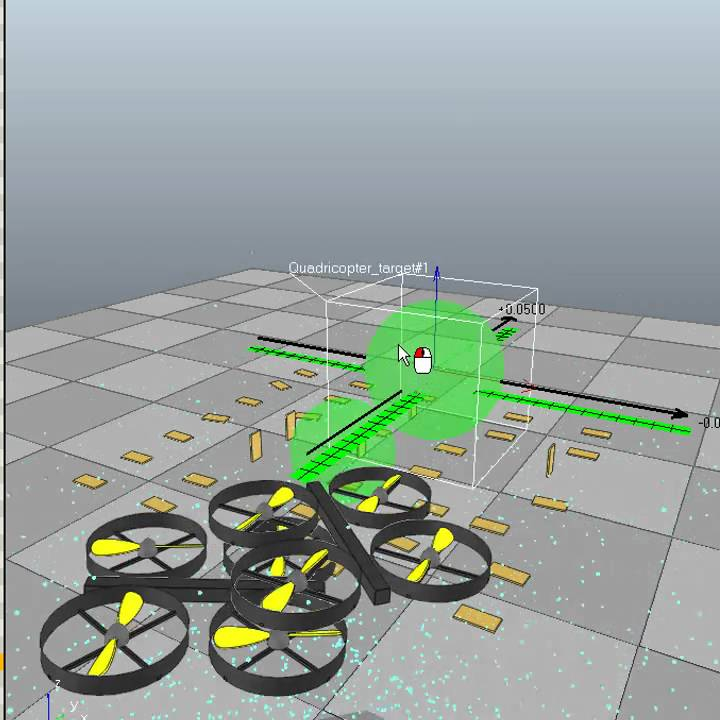
\includegraphics[width=.95\linewidth]{figures/vrep_example}
    \caption{V-Rep}
    \label{fig:vrep_example}
  \end{subfigure}%
  \begin{subfigure}{.33\textwidth}
    \centering
    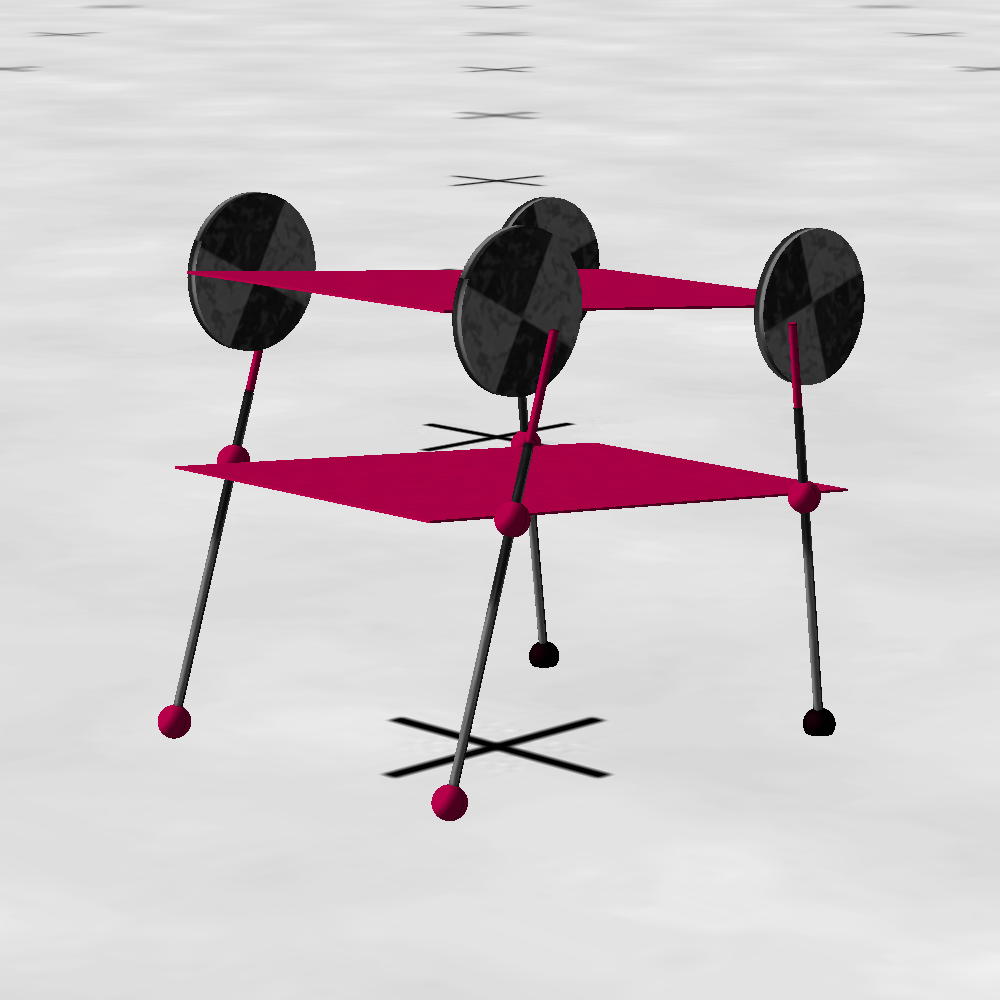
\includegraphics[width=.95\linewidth]{figures/lpzrobots_example}
    \caption{LPZ Robots}
    \label{fig:lpzrobots_example}
  \end{subfigure}
  \begin{subfigure}{.33\textwidth}
    \centering
    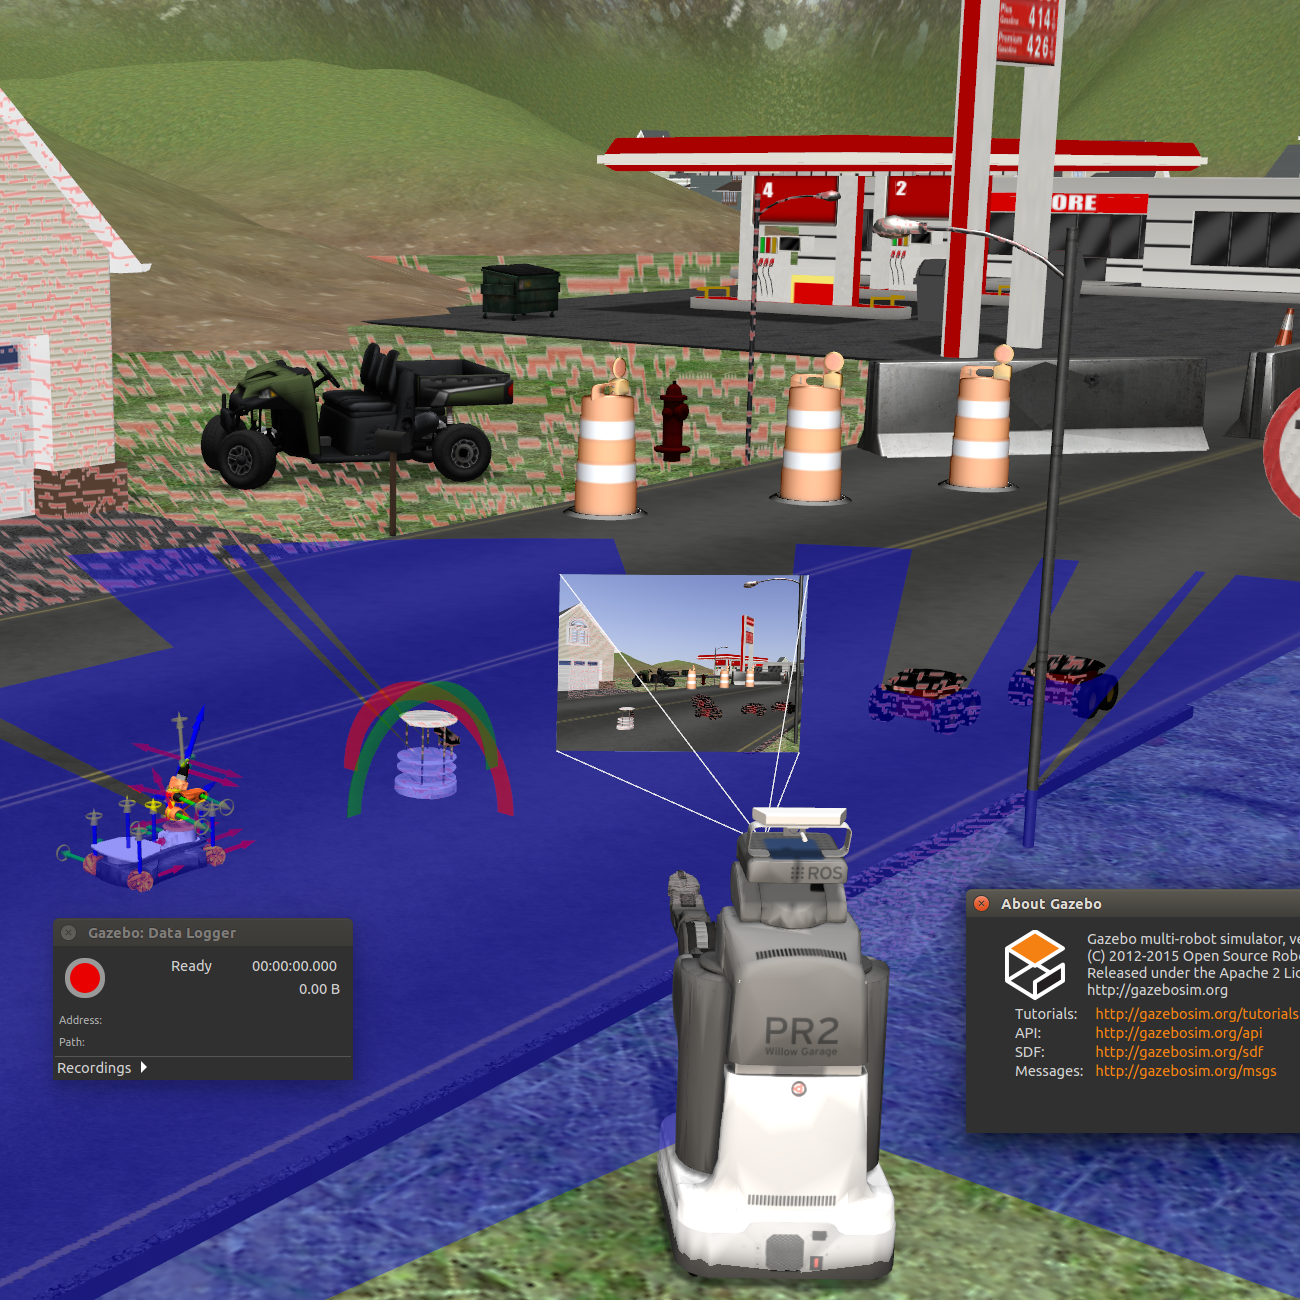
\includegraphics[width=.95\linewidth]{figures/gazebo_example}
    \caption{Gazebo}
    \label{fig:gazebo_example}
  \end{subfigure}
  \caption{Simulation examples of the software analyzed.}
  \label{fig:simulation_comparison}
\end{figure}

The RuBi robot is mainly targeted to be used in the Embodied AI \& Neurorobotics Lab at the Mærsk Mc-Kinney Møller Institute, where the toolbox GoRobots is currently being developed.
This is a kit of development tools, from a neuronal networks API to a genetic algorithm engine, written in C++ that is meant to be simulator-independent.
However, because of the reasons given in previous chapters, ROS Jade \cite{ros} has been selected as the tool to use.
The whole set of instruments provided in ROS along with its easy extendability give the opportunity to use the controllers and tools already developed in GoRobots.
Despite the fact that the three simulators compared have a C++ interface that would allow to interface them with ROS, Gazebo is already fully supported and integrated in ROS, making it the logic choice.
This reduces the learning curve of a new user and the installation process is easier due to the fact that it is included in the Open Source Robotics Foundation (OSRF) repositories.

Regarding the second condition, Gazebo has the feature of selecting the physics engine in the beginning of the simulation, it has multiphysics support (fluids, electromagnetism...), it allows to load external geometries from STL or Collada and, the most important, has an active community behind it providing support and documentation. These are the reasons for selecting Gazebo as the simulator for the RuBi platform.
In \cite{physics_engine_gazebo_comparison}, a comparison with the different physical engines is carried out.
For the sake of simplicity the default one, Open Dynamics Engine (ODE), has been used, although the others have been tested.

% section comparison_of_simulators (end)\[